\qrchapter{https://forgottenpillar.com/rsc/en-fp-chapter10}{Is God a person? - by John N. Loughborough}


\qrchapter{https://forgottenpillar.com/rsc/en-fp-chapter10}{Je, Mungu ni nafsi? - na John N. Loughborough}


One of the earliest articles on the \emcap{personality of God} is Loughborough’s article “\textit{Is God a person?}” where he discusses the \emcap{personality of God} and His presence. It is important to remember the definition of ‘personality’ according to the Merriam-Webster dictionary: “\textit{the quality or state of being a person}”\footnote{\href{https://www.merriam-webster.com/dictionary/personality}{Merriam-Webster Dictionary - ‘\textit{personality}’}}. We will look carefully at how Loughborough sees the quality or state of God being a person.


Mojawapo ya makala ya mapema zaidi juu ya \emcap{Umbile la Mungu} ni nakala ya Loughborough “\textit{Je, Mungu ni nafsi?}” ambapo anazungumzia \emcap{Umbile la Mungu} na uwepo wake. Ni muhimu kumbuka maana ya ‘personality’ kulingana na kamusi ya Merriam-Webster: “\textit{Ubora au hali ya kuwa Nafsi}”\footnote{\href{https://www.merriam-webster.com/dictionary/personality}{Merriam-Webster Dictionary - ‘\textit{personality}’}}. Tutaangalia kwa uangalifu jinsi Loughborough anavyoona ubora au hali ya Mungu kuwa Nafsi.


\begin{figure}[hp]
    \centering
    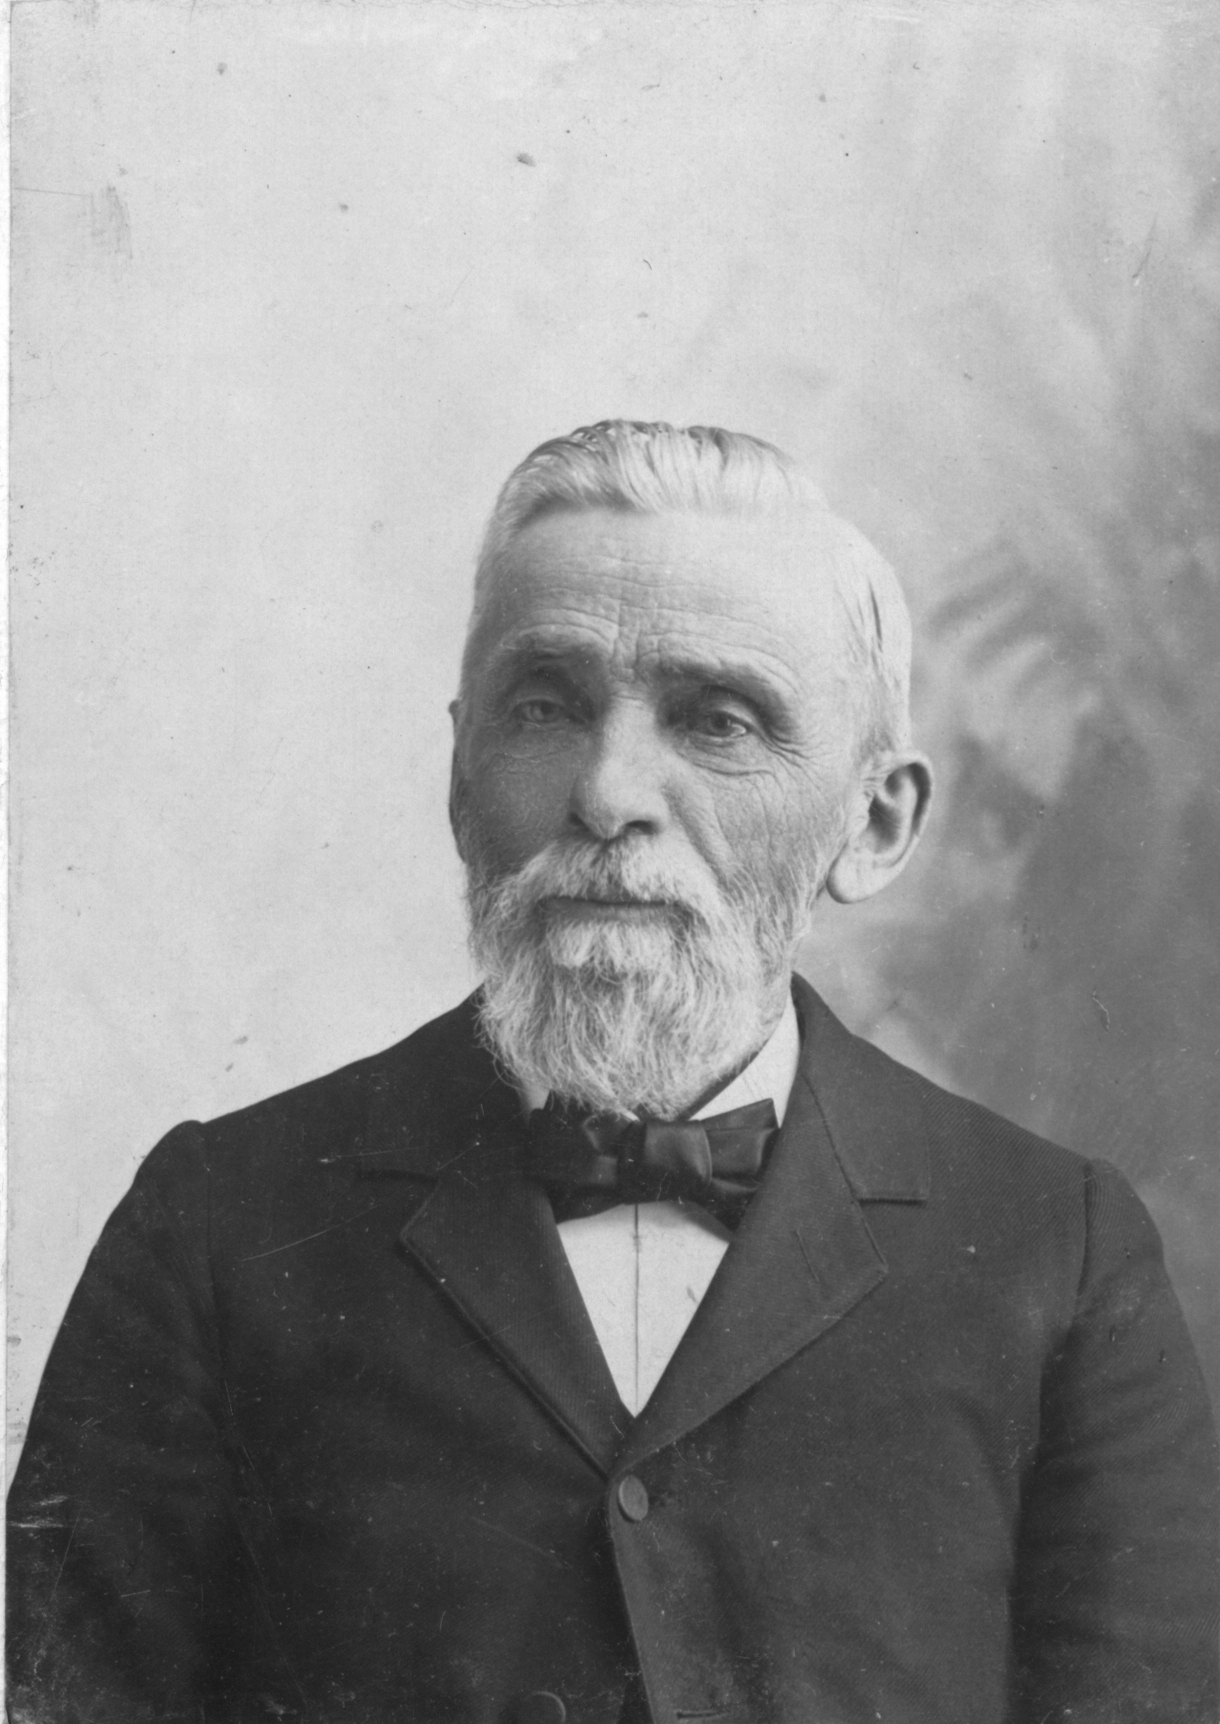
\includegraphics[width=1\linewidth]{images/john-n-loughborough.jpg}
    \caption*{John Norton Loughborough (1832-1924)}
    \label{fig:john-n-loughborough}
\end{figure}


\begin{figure}[hp]
    \centering
    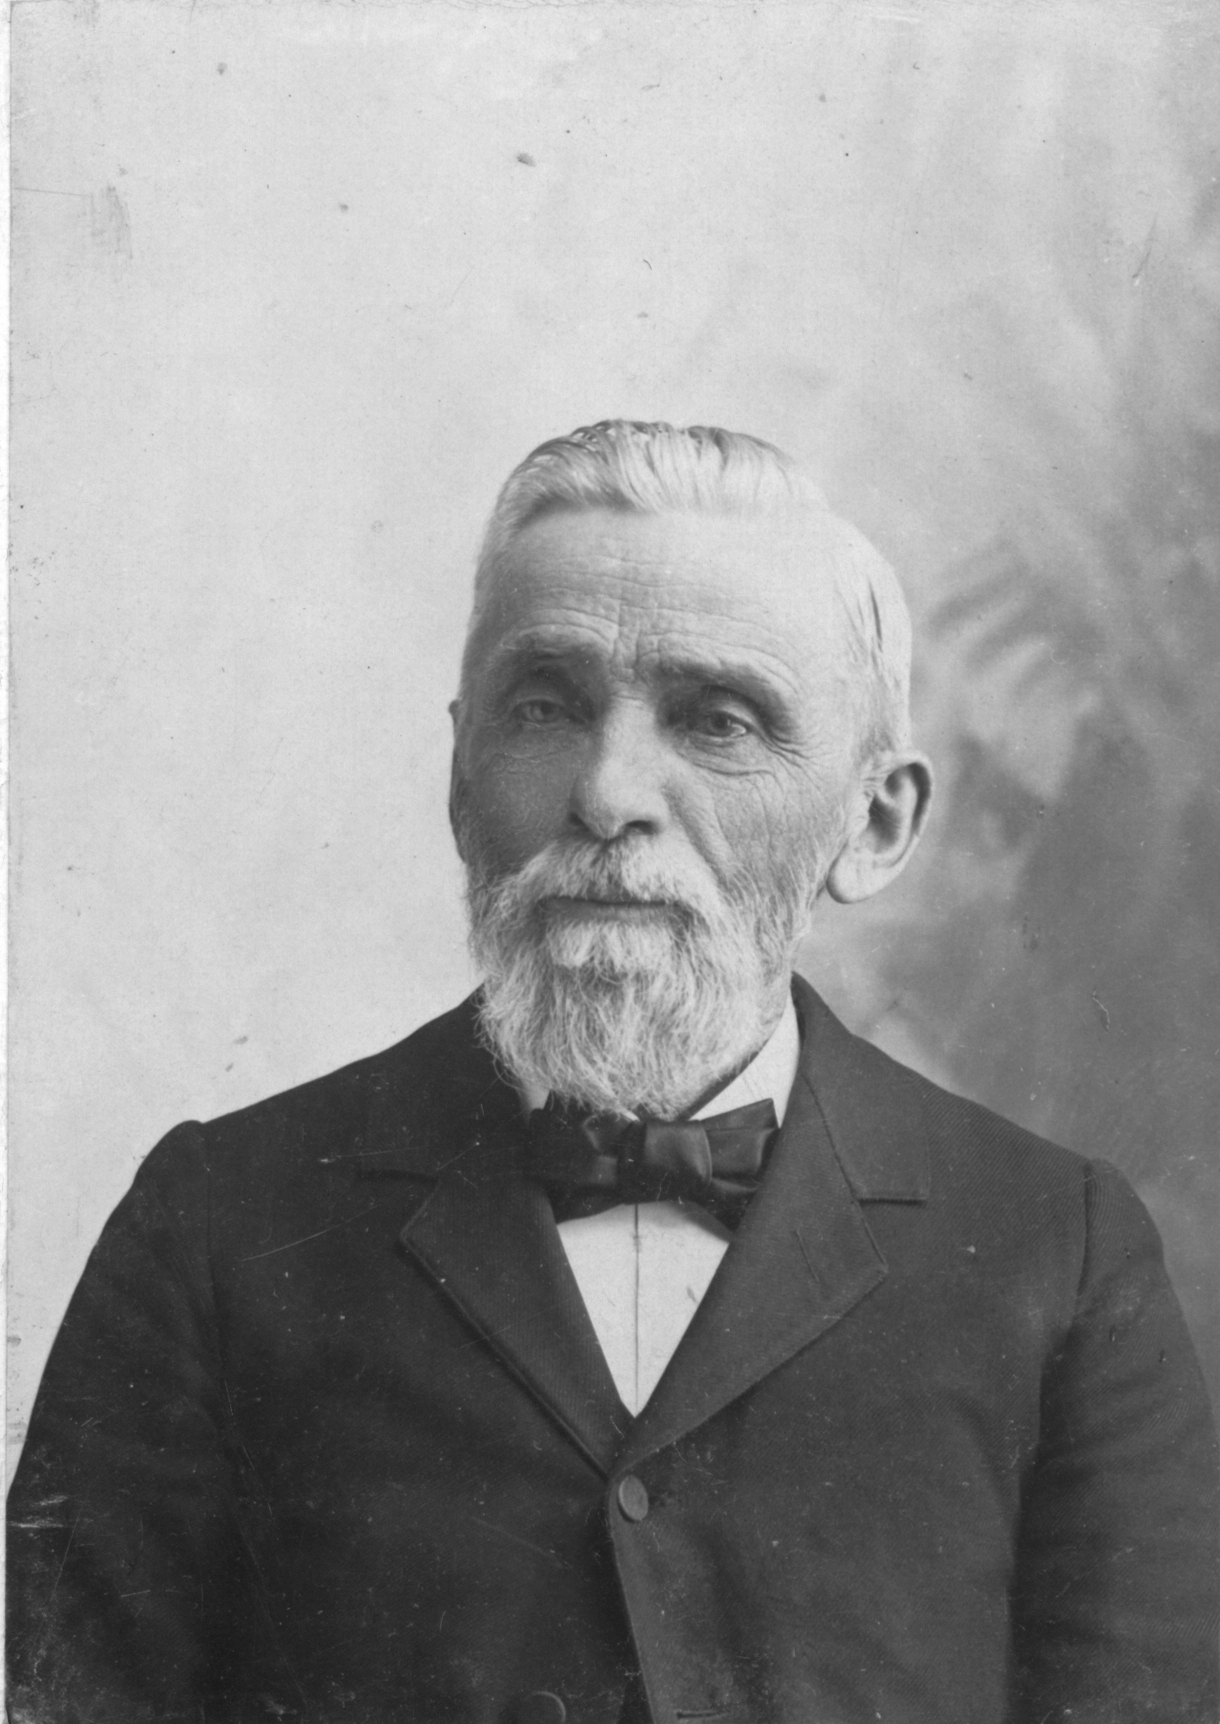
\includegraphics[width=1\linewidth]{images/john-n-loughborough.jpg}
    \caption*{John Norton Loughborough (1832-1924)}
    \label{fig:john-n-loughborough}
\end{figure}


\others{Whatever may be the truth in this matter, it certainly cannot be wrong for us to examine what the Word says respecting it. \textbf{Many there are that would refrain from the investigation of unpopular truths because the cry of heresy is raised against them}. We shall not consider ourselves subjects of the appellation, \textbf{neither are we prying into the secrets of the Almighty, as we pursue the investigation of this matter}. The Bible certainly contains testimony upon this point, and we again repeat, ‘\textbf{Things which are revealed belong to us}.’ We inquire then, What saith the Scripture?}


\others{Chochote kinachoweza kuwa ukweli katika suala hili, hakika haiwezi kuwa vibaya kwetu kuchunguza kile ambacho Neno linasema juu yake. \textbf{Kuna wengi ambao wangejiepusha na uchunguzi wa ukweli usiopendwa na watu wengi kwa sababu kilio cha uzushi kinainuliwa dhidi yao}. Sisi hatutajiona kuwa watu wa jina hilo, \textbf{wala hatujiingizi ndani ya siri za Mwenyezi, tunapofuatilia uchunguzi wa jambo hili}. Bibilia hakika ina ushuhuda juu ya jambo hili, na tunarudia tena, ‘\textbf{Vitu vilivyofunuliwa kwetu ni vyetu}.’ Tunauliza basi, Maandiko Matakatifu yasemaje?}


\othersnogap{\textbf{The very testimony we have been examining in regard to man’s being formed of the dust in \underline{the image of God}, proves conclusively that \underline{God has a form}, although the sentiment is contrary to what we have been taught, while children, from the catechism}:}


\othersnogap{\textbf{Ushuhuda wenyewe ambao tumekuwa tukichunguza kuhusu mwanadamu kuumbwa kwa mavumbi \underline{katika mfano wa Mungu}, unathibitisha kabisa kwamba \underline{Mungu ana namna}, ingawa hisia hii ni kinyume na yale tumefundishwa, tulipokuwa watoto, kutoka katekisimu}:}


\othersnogap{Question. ‘What is God?’}


\othersnogap{Swali. ‘Mungu ni nini?’}


\othersnogap{Answer. ‘An infinite and eternal spirit; one that always was and always will be.’}


\othersnogap{Jibu. ‘Roho isiyo na mwisho na ya milele; moja ambayo sikuzote ilikuwako na itakuwako daima.’}


\othersnogap{Q. ‘Where is God?’}


\othersnogap{Swali. ‘Mungu yuko wapi?’}


\othersnogap{A. ‘Everywhere.’}


\othersnogap{Jibu. ‘Kila mahali.’}


\othersnogap{\textbf{But we inquire, \underline{Is not God in one place more than another}?} Oh no, say you: \textbf{the Bible says \underline{he is a spirit}, and if so he must be \underline{everywhere alike}}. Well, if when man dies his spirit goes to God, it must go everywhere. \textbf{But the Bible certainly represents God as located in heaven. ‘For he hath looked down from the height of his sanctuary: from heaven did the Lord behold the earth.’ Psalm 102:19}. \textbf{Then certainly heaven cannot be everywhere, for God is represented as looking down from it. ‘\underline{Elijah went up} by a whirlwind \underline{into heaven}.’ 2 Kings 2:11}. \textbf{But, says one, does not the Bible represent God \underline{as everywhere present}?} Psalm 139:8, 9, 10. ‘If I ascend up into heaven, \textbf{thou art there}: if I make my bed in hell, \textbf{behold, thou art there}; if I take the wings of the morning, and dwell in the uttermost parts of the sea,\textbf{ even there shall thy hand lead me}, and thy right hand shall hold me.’}


\othersnogap{\textbf{Lakini tunauliza, \underline{Je! Hayuko Mungu mahali pamoja kuliko pengine}?} La hasha, unasema: \textbf{Biblia inasema \underline{yeye ni roho}, na ikiwa hivyo lazima awe \underline{kila mahali sawia}}. Vema, ikiwa mwanadamu anapokufa roho yake inaenda kwa Mungu, lazima iende kila mahali. \textbf{Lakini Biblia hakika inamwakilisha Mungu kama kupatikana mbinguni. ‘Kwa maana ametazama kutoka mahali palipoinuka patakatifu pake: kutoka mbingu Bwana aliitazama nchi.’ Zaburi 102:19}. \textbf{Basi hakika mbinguni haiwezi kuwa kila mahali, kwa maana Mungu anawakilishwa kama anatazama chini kutoka humo. ‘\underline{Eliya akapanda juu} na kimbunga \underline{mbinguni}.’ 2 Wafalme 2:11}. \textbf{Lakini, asema mmoja, si Biblia humwakilisha Mungu \underline{kuwepo kila pahali}?} Zaburi 139:8, 9, 10. ‘Nikipanda mbinguni, \textbf{wewe uko pale}: nikitandika kitanda changu kuzimu, \textbf{tazama, uko huko}; nikishika mbawa za asubuhi, na kukaa ndani ya pande za mwisho za bahari, \textbf{hata huko mkono wako utaniongoza}, na mkono wako wa kuume utanishika.’}


\othersnogap{We reply, \textbf{the subject is introduced in verse 7, as follows}: ‘\textbf{\underline{Whither shall I go from thy Spirit}?} \textbf{or whither shall I flee from \underline{thy presence}?}’ \textbf{The Spirit is \underline{God’s representative}}. \textbf{His power is manifested wherever he listeth, through the agency of his Spirit}. Christ, when giving the commission to the disciples, says, ‘Go ye into all the world, and preach the gospel to every creature, and lo! \textbf{I am with you alway, even unto the end of the world}.’ Now, no one would contend that Christ had been on the earth personally ever since the disciples commenced to fulfill this commission. \textbf{But his Spirit has been on the earth; the Comforter that he promised to send.} \textbf{So in the same manner God manifests himself \underline{by his Spirit} which is also the power through which he works}. ‘But if \textbf{the Spirit of him} that raised up Jesus from the dead dwell in you, \textbf{he that raised up Christ} from the dead shall also quicken your mortal bodies \textbf{\underline{by his Spirit} that dwelleth in you}.’ Romans 8:11. \textbf{\underline{Here is a plain distinction made between the Spirit, and God that raises the dead by that Spirit}}. \textbf{If the living God is a Spirit in the strictest sense of the term, and at the same time is in possession of a Spirit, then we have at once the novel idea of the Spirit of a Spirit, something it will take at least a Spiritualist to explain}.}[The Adventist Review and Sabbath Herald, September 18, 1855][https://documents.adventistarchives.org/Periodicals/RH/RH18550918-V07-06.pdf]


\othersnogap{Tunajibu, \textbf{somo limeanzishwa katika mstari wa 7, kama ifuatavyo}: ‘\textbf{\underline{Nitaenda wapi kutoka kwa Roho yako}?} \textbf{au nitakimbilia wapi kutoka kwa \underline{uwepo wako}?}’ \textbf{Roho ni \underline{mwakilishi wa Mungu}}. \textbf{Nguvu zake hudhihirika popote anapotaka, kupitia wakala wa Roho wake}. Kristo, anapowapa wanafunzi agizo, anasema, ‘Enendeni ulimwenguni mwote, mkahubiri Injili kwa kila kiumbe, na hakika! \textbf{Niko pamoja nanyi siku zote, hata hadi mwisho wa dahari}.’ Sasa, hakuna mtu ambaye angepinga kwamba Kristo amekuwa duniani kibinafsi tangu wakati wanafunzi wake walianza kutimiza agizo hili. \textbf{Lakini Roho wake amekuwa juu ya nchi; Mfariji ambaye aliahidi kutuma.} \textbf{Hivyo kwa namna hiyo hiyo Mungu hujidhihirisha \underline{kupitia kwa Roho yake} ambayo pia ni nguvu ambayo kwayo anafanya kazi}. ‘Lakini ikiwa \textbf{Roho wa huyo} aliyemfufua Yesu kutoka kwa wafu atakaa ndani yenu, \textbf{yeye aliyemfufua Kristo} kutoka kwa wafu atahuisha miili yenu iliyo katika hali ya kufa \textbf{\underline{kwa Roho wake} akaaye ndani yenu}.’ Warumi 8:11. \textbf{\underline{Hapa kuna utofauti wa wazi kati ya Roho, na Mungu ambaye huwafufua wafu kwa Roho huyo}}. \textbf{Ikiwa Mungu aliye hai ni Roho kwa maana kali ya neno, na wakati huo huo anamiliki Roho, basi tunapata wazo jipya la Roho wa Roho, jambo ambalo litamhitaji angalau Mmizimu kueleza}.}[The Adventist Review and Sabbath Herald, September 18, 1855][https://documents.adventistarchives.org/Periodicals/RH/RH18550918-V07-06.pdf]


Allow us to make a short comment. We hope you recognize the specific topic being discussed here. The subject is the first point of the \emcap{Fundamental Principles} and the assertion is that God does have a form, for man is made in the image of God. Such understanding of God’s personality precludes the idea that God is everywhere present. Brother Loughborough gave the biblical reasons for God's omnipresence, together with the sentiment that “\textit{God is in one place more than another}”. God is everywhere present by His representative, the Holy Spirit, just as it is written in the first point of the \emcap{Fundamental Principles}. Further in this discussion, we will read that God is a spiritual being and possesses a tangible, material body, in contrast to the idea that He is purely a spirit.


Turuhusu tutoe maoni mafupi. Tunatumahi unatambua mada mahususi inayojadiliwa hapa. Somo ni hoja ya kwanza ya \emcap{Kanuni za Msingi} na madai ni kwamba Mungu ana namna, kwa maana mwanadamu ameumbwa kwa mfano wa Mungu. Uelewa kama huo wa ubinafsi wa Mungu huzuia wazo la kwamba Mungu yuko kila mahali. Ndugu Loughborough alitoa sababu za kibiblia za uwepo wa Mungu kila mahali, pamoja na maoni kwamba “\textit{Mungu yuko katika sehemu moja zaidi ya nyingine}”. Mungu yuko kila mahali kupitia kwa mwakilishi wake, Roho Mtakatifu, kama ilivyoandikwa katika hoja ya kwanza ya \emcap{Kanuni za Msingi}. Zaidi katika majadiliano haya, tutasoma kwamba Mungu ni huluki ya kiroho na anamiliki mwili unaoonekana na kushikika, tofauti na wazo kwamba Yeye ni roho tu.


\others{There is at least one impassable difficulty in the way of \textbf{those who believe \underline{God is immaterial}, and heaven is not a literal, \underline{located place}: they are obliged to admit that \underline{Jesus is there bodily, a literal person}}; the same Jesus that was crucified, dead, and buried, was raised from the dead, \textbf{ascended up to heaven}, and is now \textbf{at the right hand of God}. \textbf{Jesus was possessed of flesh and bones after his resurrection}. Luke 24:39. ‘\textbf{Behold my hands and my feet, that it is I, myself; handle me, and see; \underline{for a spirit hath not flesh and bones as ye see me have}}.’ \textbf{If Jesus is there in heaven with a literal body of flesh and bones, may not heaven after all be a literal place, a habitation for a literal God, a literal Saviour, literal angels, and resurrected immortal saints?} \textbf{\underline{Oh no, says one, ‘God is a Spirit.’}} So Christ said to the woman of Samaria at the well. \textbf{It does not necessarily follow because God is a Spirit, \underline{that he has no body}}. In John 3:6, Christ says to Nicodemus, ‘\textbf{That which is born of the Spirit is spirit}.’ \textbf{If that which is born of the Spirit is spirit, then on the same principle, that which has a spiritual nature is spirit. God is \underline{a spirit being}, his nature is spirit, he is not of a mortal nature; }\textbf{\underline{but this does not exclude the idea of his having a body}}. David says, [Psalm 114:4,] ‘Who maketh \textbf{his angels spirits};’ yet \textbf{\underline{angels have bodies}}. Angels appeared to both Abraham and Lot, and ate with them. \textbf{We see the idea that angels are spirits, does not prove that they are not literal beings}.}


\others{Kuna angalau ugumu mmoja usiopitika katika njia ya \textbf{wale wanaomwamini \underline{Mungu anakosa mwili}, na mbingu si mahali halisi, panapo-dhihirika: wanalazimika kukubali kwamba \underline{Yesu yuko pale kimwili, nafsi halisi}}; Yesu yule yule aliyesulubiwa, akafa, na akazikwa, akafufuliwa kutoka kwa wafu, \textbf{akapaa juu mbinguni}, na sasa yuko \textbf{upande wa mkono wa kuume wa Mungu}. \textbf{Yesu alimiliki nyama na mifupa baada ya kufufuka kwake}. Luka 24:39. ‘\textbf{Tazameni mikono yangu na miguu yangu, ya kuwa ni mimi mwenyewe; nishikeni, mwone; \underline{kwa maana roho haina nyama na mifupa kama mnionavyo kuwa nayo}}.’ \textbf{Ikiwa Yesu yuko mbinguni akiwa na mwili halisi ya nyama na mifupa, hata mbinguni isiwe mahali halisi, makao ya halisi Mungu, Mwokozi halisi, malaika halisi, na watakatifu waliofufuliwa wasioweza kufa?} \textbf{\underline{Hapana, anasema moja, ‘Mungu ni Roho.’}} Ndivyo Kristo alimwambia mwanamke Msamaria kwenye kisima. \textbf{Haifuatii kuwa ulazima eti kwa sababu Mungu ni Roho, \underline{kwamba hana mwili}}. Katika Yohana 3:6, Kristo anamwambia Nikodemo, ‘\textbf{Kilichozaliwa kwa Roho ni roho}.’ \textbf{Ikiwa kile kilichozaliwa na Roho ni roho, basi kwa kanuni hiyo hiyo, kilicho na asili ya kiroho ni roho. Mungu ni \underline{huluki roho}, asili yake ni roho, yeye si wa mwili wa kufa; }\textbf{\underline{lakini hii haiondoi wazo la yeye kuwa na mwili}}. Daudi asema, [Zaburi 114:4,] ‘Ni nani afanyaye \textbf{malaika wake roho};’ bado \textbf{\underline{malaika wana miili}}. Malaika waliwatokea Ibrahimu na Lutu, na wakakula nao. \textbf{Tunaona wazo la kwamba malaika ni roho, halithibitishi kwamba si viumbe halisi}.}


\othersnogap{It is inferred because the Bible says that God is a Spirit, that he is not a person. An inference should not be made the basis for an argument. Great Scripture truths are plainly stated, and it will not do for us to found a doctrine on inferences, \textbf{contrary to positive statements in the word of God}. If the Scripture states in positive \textbf{terms that God is a person, it will not answer for us to draw an inference from the text which says ‘God is a Spirit,’ \underline{that he has no body}}.}


\othersnogap{Imefikiriwa kwa sababu Biblia inasema kwamba Mungu ni Roho, eti yeye si nafsi. Mtazamo haupaswi kuwa msingi wa hoja. Kweli kuu za Maandiko zinasemwa wazi, na haitaufanyia kuunda fundisho juu ya makisio, \textbf{kinyume na kauli chanya katika neno la Mungu}. Ikiwa Maandiko yanasema kwa maneno chanya \textbf{kwamba Mungu ni nafsi, haitakuwa jibu kwetu kuchukua hitimisho kutoka kwa kifungu kinachosema ‘Mungu ni Roho,’ \underline{kwamba yeye hana mwili}}.}


\othersnogap{We will now present a few texts \textbf{which prove that God is a person}. Exodus 33:18, 23. ‘And he (Moses) said, I beseech thee shew me thy glory.’ Verse 20. ‘And he said, \textbf{Thou canst not see \underline{my face}, for there shall no man see me and live}.’ Verses 21-23. ‘And the Lord said, Behold there is a place by me, and thou shalt stand upon a rock: and it shall come to pass while my glory passeth by, that I will put thee in a cleft of the rock; and \textbf{will cover thee with \underline{my hand} while I pass by}; and I will take away \textbf{mine hand}, and thou shalt \textbf{see my \underline{back parts}}; but \textbf{\underline{my face} shall not be seen.’} \textbf{If God is \underline{an immaterial Spirit}, then Moses could not see him; for we are told a spirit cannot be seen by natural eyes}. \textbf{There would then be no propriety for God to say he would put his hand over Moses’ face while he passed by, (seemingly to prevent him from seeing his face,) for he could not see him}. Neither do we conceive how an immaterial hand could obstruct the rays of light from passing to Moses’ eyes. \textbf{But if the position be true \underline{that God is immaterial}, and cannot be seen by the natural eye, the text above is all superfluous}. \textbf{What sense is there in saying God put his hand over Moses’ face, to prevent him from seeing that which could not be seen}.}


\othersnogap{Sasa tutawasilisha vifungu vichache \textbf{vinavyothibitisha kwamba Mungu ni nafsi}. Kutoka 33:18, 23. ‘Na yeye (Musa) akasema, nakuomba unionyeshe utukufu wako.’ Aya 20. ‘Na akamwambia, \textbf{Huwezi ona \underline{uso wangu}, kwa maana hakuna mtu atakayeniona na kuishi}.’ Mstari wa 21-23. ‘Bwana akasema, Tazama, kuna mahali karibu nami, nawe utasimama juu ya mwamba: na itatimia wakati utukufu wangu utapita, nitakuweka katika ufa wa mwamba; na \textbf{nitakufunika na \underline{mkono wangu} nipitapo}; nami nitauondoa \textbf{mkono wangu}, nawe utaniona \textbf{sehemu zangu za \underline{nyuma}}; lakini \textbf{\underline{uso wangu} hautaonekana.’} \textbf{Ikiwa Mungu ni \underline{Roho asiye na mwili}, basi Musa asingeweza kumwona; kwa maana tunaambiwa roho haiwezi kuonekana kwa macho ya kawaida}. \textbf{Basi Mungu asingekuwa mwenye haki kusema kwamba angeweka mkono wake juu ya uso wa Musa wakati yeye angepita (ikionekana kumzuia asiuone uso wake), kwa maana hakuweza kumwona}. Wala hatufikirii jinsi mkono usio na mwili unavyoweza kuzuia miale ya mwanga kupita kwa macho ya Musa. \textbf{Lakini ikiwa msimamo huo ni wa kweli \underline{kwamba Mungu hana mwili}, na hawezi kuonekana kwa jicho la kawaida, maandishi ya hapo juu yote ni yasiyohitajiwa}. \textbf{Kuna maana gani ya kusema Mungu akaweka mkono wake juu ya uso wa Musa, ili kumzuia asione kile ambacho hakiwezi kuonekana}.}


\othersnogap{Says one, I see we cannot harmonize the matter any other way, than that there was a literal body seen by Moses; but that was not God’s own body, \textbf{it was a body he took that he might show himself to Moses}. \textbf{Moses could form no just conceptions of God unless he assumed a form.} \textbf{So God took a body}. This throws a worse coloring on the matter than the first position; \textbf{for it charges God with deception; telling Moses he should see him, when in fact Moses according to this testimony did not see God, but another body}. A person must be given to doubt almost beyond recovery, that would attempt thus to mystify, and do away the force of this testimony.}[Ibid.][https://documents.adventistarchives.org/Periodicals/RH/RH18550918-V07-06.pdf]


\othersnogap{Anasema mmoja, naona hatuwezi kuoanisha jambo hilo kwa njia nyingine yoyote, isipokuwa kwamba kulikuwa na mwili halisi ulioonekana na Musa; lakini huo haukuwa mwili wa Mungu mwenyewe, \textbf{bali ni mwili alioutwaa ili aweze kujionyesha kwa Musa}. \textbf{Musa hakuweza kuunda dhana za haki za Mungu isipokuwa tu alichukua fomu.} \textbf{Kwa hiyo Mungu akatwaa mwili}. Hii inatupa rangi mbaya zaidi juu ya jambo hilo kuliko nafasi iliyotolewa ya kwanza; \textbf{kwa maana inamsingizia Mungu udanganyifu; kumwambia Musa amwone, wakati kwa hakika Musa kulingana na ushuhuda huu hakuona Mungu, bali mwili mwingine}. Mtu lazima apeanwe kwa shaka karibu zaidi ya kupona, ambayo ingejaribu kuficha, na kuondoa nguvu ya ushuhuda huu.}[Ibid.][https://documents.adventistarchives.org/Periodicals/RH/RH18550918-V07-06.pdf]


Do you recognize that Brother Loughborough is tackling the sentiment that Dr. Kellogg would present in the Living Temple 48 years later? Dr. Kellogg said that it is true that God presented Himself in a\others{\textbf{\underline{particular form or place}}}[Dr. John H. Kellogg, The Living Temple, p.31.][https://archive.org/details/J.H.Kellogg.TheLivingTemple1903/page/n31/] because \others{there must be something more \textbf{tangible}, more \textbf{\underline{restricted}}, upon which to center the mind in worship}[bid, p.30][https://archive.org/details/J.H.Kellogg.TheLivingTemple1903/page/n30/], but that He is, in reality,\others{\textbf{far beyond our comprehension \underline{as are the bounds of space and time}}}[Ibid, p.33][https://archive.org/details/J.H.Kellogg.TheLivingTemple1903/page/n33/]. Brother Loughborough reasonably objected to the idea that God is only manifesting Himself to man as a definite Being, but in reality, is not what He presents Himself to be. Such a claim\others{charges God with deception}. Brother Loughborough continues with the affirmative, Biblical testimony that God is a material being.


Je, unatambua kwamba Ndugu Loughborough anashughulikia hisia ambazo Dk. Kellogg angewasilisha katika Hekalu Hai miaka 48 baadaye? Dk. Kellogg alisema kwamba ni kweli kwamba Mungu alijidhihirisha katika\others{\textbf{\underline{namna au mahali maalum}}}[Dr. John H. Kellogg, The Living Temple, p.31.][https://archive.org/details/J.H.Kellogg.TheLivingTemple1903/page/n31/] kwa sababu \others{lazima kuwe na kitu kinachoshikika zaidi, \textbf{\underline{kinachozuiliwa}} zaidi, ambacho juu yake kitaweka akili katika ibada}[bid, p.30][https://archive.org/details/J.H.Kellogg.TheLivingTemple1903/page/n30/], lakini kwamba Yeye yuko, kwa kweli,\others{\textbf{mbali zaidi ya ufahamu wetu \underline{kama ilivyo mipaka ya nafasi na wakati}}}[Ibid, p.33][https://archive.org/details/J.H.Kellogg.TheLivingTemple1903/page/n33/]. Ndugu Loughborough alipinga wazo la kwamba Mungu anajidhihirisha tu kwa mwanadamu kama huluki dhahiri, lakini kwa uhalisi, si kile anachojionyesha kuwa. Madai kama hayo\others{humshtaki Mungu kwa udanganyifu}. Ndugu Loughborough anaendelea na uthibitisho wa hakika, wa ushuhuda wa Kibiblia kwamba Mungu ni huluki mwenye mwili.


\others{Exodus 24:9. ‘Then went up Moses and Aaron, Nadab and Abihu, and seventy of the elders of Israel: \textbf{and they saw the God of Israel}: and there was under \textbf{his feet} as it were a paved work of a sapphire stone, and as it were the body of heaven in its clearness.’ They were permitted to \textbf{see his feet}, but no \textbf{man can see his face and live}. \textbf{No \underline{mortal eye} can bear the dazzling brightness of that glory of the face of God}. It far exceeds the light of the sun. For the prophet says, ‘The light of the moon shall be as the light of the sun, and the light of the sun shall be \textbf{seven fold}, as the light of seven days, in the day that the Lord bindeth up the breach of his people, and healeth the stroke of their wound.’ Isaiah 30:26. Notwithstanding this seven-fold light that is then to shine, the prophet speaking of the scene says, ‘Then the moon shall be confounded, and the sun ashamed, when the Lord of hosts shall reign in mount Zion, and in Jerusalem, and before his ancients gloriously.’ Isaiah 24:23. The testimony of John is, [Revelation 21:23,] ‘And the city had no need of the sun, neither of the moon, to shine in it: for \textbf{the glory of God did lighten it,} and the Lamb is the light thereof.’}


\others{Kutoka 24:9. ‘Basi wakaenda juu Musa, na Haruni, Nadabu na Abihu, na wazee sabini wa Israeli: \textbf{nao wakamwona Mungu wa Israeli}: na pale chini ya \textbf{miguu yake} palikuwa kama sakafu kazi ya samawi, na kama ilivyokuwa mwili wa mbinguni katika uangavu wake.’ Waliruhusiwa kuona \textbf{miguu yake}, lakini hakuna \textbf{mtu awezaye kuuona uso wake na kuishi}. \textbf{Hakuna \underline{jicho la mwanadamu} linaloweza kustahimili mng'ao unaong'aa wa utukufu ule wa uso wa Mungu}. Inazidi sana nuru ya jua. Kwa maana nabii asema, ‘Nuru ya mwezi itakuwa kama nuru ya jua, na mwanga wa jua utakuwa \textbf{mara saba}, kama nuru ya siku saba, katika siku hiyo Bwana afungapo jeraha la watu wake, na kuponya mapigo ya jeraha yao.’ Isaya 30:26. Bila Kujali nuru hii ya mara saba ambayo itaangaza, nabii akinena juu ya tukio hilo asema, ‘Ndipo mwezi utatahayarika, na jua litaaibika, wakati Bwana wa majeshi atatawala katika mlima Sayuni, na katika Yerusalemu, na mbele ya wazee wake kwa utukufu.’ Isaya 24:23. Ushuhuda wa Yohana ni, [Ufunuo 21:23,] ‘Na mji ule hauhitaji jua, wala mwezi, uangaze ndani yake: kwa maana \textbf{utukufu wa Mungu huutia nuru,} na nuru ni Mwana-Kondoo yake.’}


\othersnogap{\textbf{Infidels claim that there is a contradiction in the testimony of Moses, because he said, he talked with God face to face}. \textbf{We reply, there was a cloud between them}, but God told Moses, ‘\textbf{No man shall see me and live}.’ The Testimony of the New Testament is in harmony with that of the Old upon this subject. ‘Follow peace with all men, and holiness without which \textbf{no man shall see the Lord}.’ Hebrews 12:14. \textbf{Who with \underline{mortal eyes} could behold a light that far outshines seven fold the brightness of the sun?} Surely none but the holy can behold him, \textbf{none but immortal eyes} could bear that radiant glory. Although the Word says we cannot see God now and live, the promise is, that the \textbf{pure in heart shall see him}. Matthew 5:3. ‘Blessed are the pure in heart, \textbf{for they shall see God}.’ Revelation 22:4. ‘And \textbf{they shall see his face}, and his name shall be in their foreheads.’}


\othersnogap{\textbf{Makafiri wanadai kuwa kuna ukinzani katika ushahidi wa Musa, kwa sababu alisema: alizungumza na Mungu uso kwa uso}. \textbf{Sisi tunajibu, palikuwa na wingu baina yao}, lakini Mwenyezi Mungu alimwambia Musa, ‘\textbf{Hakuna mtu atakayeniona na kuishi}.’ Ushuhuda wa Agano Jipya na lile la Kale linauwiano juu ya somo hili. ‘Fuata amani na watu wote, na utakatifu bila hayo \textbf{hakuna mtu atakayemwona Bwana}.’ Waebrania 12:14. \textbf{Nani kwa \underline{macho ya kufa} anaweza kutazama nuru iangazayo zaidi ya mara saba ya mwangaza wa jua?} Hakika hakuna lakini watakatifu wanaweza kumwona, \textbf{hakuna ila macho yasiyoweza kufa} yangeweza kustahimili utukufu wa ule mngao. Ingawa Neno linasema hatuwezi kumwona Mungu sasa na kuishi, ahadi ni kwamba, \textbf{wenye mioyo safi watamwona}. Mathayo 5:3. ‘Heri wenye mioyo safi, \textbf{maana hao watamwona Mungu}.’ Ufu 22:4. ‘Nao \textbf{watauona uso wake}, na jina lake litakuwa katika vipaji vya nyuso zao.’}


\othersnogap{Paul, [Colossians 1:15,] speaking of Christ, says, ‘Who is the image of \textbf{the invisible God}, the first born of every creature.’ Here Christ is said to be ‘\textbf{the image of the invisible God}.’ We have already shown, that\textbf{ Christ has a body composed of substance, flesh and bones; and he is said to be}, ‘\textbf{the image of the invisible God}.’ Well, says one, we admit his divine nature is in the image of God. If by his divine nature you mean the part that existed in glory with the Father before the world was, we reply, that which was in the beginning with God, (the Word,) \textbf{was made flesh, not came into flesh}, or as some state, \textbf{clothed upon with a human nature, but made flesh}. But says another, \textbf{God is said to be invisible}. \textbf{Because he is invisible now, it does not prove that he never will be seen}. The Word says, ‘The pure in heart \textbf{shall see him}’. Willing faith says, Amen.}


\othersnogap{Paulo, [Wakolosai 1:15,] akinena juu ya Kristo, asema, ‘Naye ni mfano wa \textbf{Mungu asiyeonekana kwetu}, mzaliwa wa kwanza wa kila kiumbe.’ Hapa Kristo anasemwa kuwa ‘\textbf{mfano wa Mungu asiyeonekana kwetu}.’ Tayari tumeonyesha, kwamba\textbf{ Kristo ana mwili unaojumuisha dutu, mwili na mifupa; naye anasemwa kuwa}, ‘\textbf{mfano wa Mungu asiyeonekana kwetu}.’ Vema, asema mmoja, twakubali asili yake ya kimungu iko katika mfano wa Mungu. Ikiwa kwa asili yake ya kimungu unamaanisha sehemu iliyokuwepo katika utukufu pamoja na Baba kabla ya ulimwengu kuwako, twajibu, kile kilichokuwa hapo mwanzo na Mungu, (Neno,) \textbf{lilifanyika mwili, si kuja katika mwili}, au kama wengine husema, \textbf{kuvikwa na asili ya kibinadamu, lakini kufanyika mwili}. Lakini mwingine anasema, \textbf{Mungu anasemwa kuwa haonekani}. \textbf{Kwa sababu haonekani sasa, haithibitishi kwamba hataonekana kamwe}. Neno linasema, ‘Wenye moyo safi \textbf{watamwona}’. Imani iliyo tayari husema, Amina.}


\othersnogap{Paul’s testimony in Philippians 2:5, 6, shows plainly what may be understood by the statement, that Christ is the image of God. ‘Let this mind be in you which was in Christ Jesus: who \textbf{being in the form of God}, thought it not robbery to \textbf{be equal with God}.’ \textbf{How can Christ be said to be in the form of God, if God has no form?} Romans 8:3. ‘God sending his own Son in the likeness of sinful flesh.’ \textbf{Christ is in the form of God, and in the form of men. This at once reveals to us the form of God}.}


\othersnogap{Ushuhuda wa Paulo katika Wafilipi 2:5, 6, unaonyesha wazi kile kinachoweza kueleweka kwa taarifa, kwamba Kristo ni mfano wa Mungu. ‘Iweni na nia iyo hiyo ndani yenu ambayo ilikuwa ndani ya Kristo Yesu: ambaye \textbf{alikuwa yuna namna ya Mungu}, hakuona kuwa sawa na Mungu kuwa ni unyang'anyi.’ \textbf{Jinsi gani Kristo anaweza kusemwa kuwa katika namna ya Mungu, ikiwa Mungu hana namna?} Warumi 8:3. ‘Mungu akimtuma Mwana wake mwenyewe katika mfano wa mwili ulio wa dhambi.’ \textbf{Kristo yu katika namna ya Mungu, na katika namna ya kibinadamu. Hii mara moja inatufunulia namna ya Mungu}.}


\othersnogap{\textbf{\underline{Daniel speaking of God, calls him the Ancient of days}}. Daniel 7:9. ‘And the Ancient of days did sit, \textbf{whose garment was white as snow}, and \textbf{the hair of his head} like the pure wool.’ \textbf{This personage is said to have a head, and hair; this certainly could not be said of him} \textbf{\underline{if he was immaterial and had no form}}. \textbf{But Paul’s testimony in \underline{Hebrews 1:3}, ought to settle every candid mind in \underline{regard to the personality of God}}. Speaking of Christ, he says, ‘Who being the brightness of his glory, \textbf{and the express image of his (the \underline{Father’s person})}.’ \textbf{Here then it is plainly stated \underline{God has a person}. Christ is the express image of it.} Then we can understand Christ where he says, ‘\textbf{He that hath seen me, hath seen the Father}.’ John 14:19. \textbf{He could not have meant, that he was his own father; for when he prayed he addressed his Father as another person who had sent him into the world}. He styled himself \textbf{the Son of God}. \textbf{Then he could not be the Father of which he was the son}. When he says, ‘He that hath seen me hath seen the Father,’ he must mean, that as \textbf{he was the express image of the Father’s person, those who saw him saw the likeness of the Father in him}.}[The Adventist Review and Sabbath Herald, September 18, 1855][https://documents.adventistarchives.org/Periodicals/RH/RH18550918-V07-06.pdf]


\othersnogap{\textbf{\underline{Danieli akinena juu ya Mungu, anamwita Mzee wa siku}}. Danieli 7:9. ‘Na Mzee wa Siku nyingi aliketi, \textbf{ambaye vazi lake lilikuwa jeupe kama theluji}, na \textbf{nywele za kichwa chake} kama safi sufu.’ \textbf{Nafsi husika anasemekana kuwa na kichwa, na nywele; hili hakika lisingeweza kusemwa kwake} \textbf{\underline{ikiwa hakuwa na mwili na hana namna}}. \textbf{Lakini ushuhuda wa Paulo katika \underline{Waebrania 1:3}, unapaswa kusuluhisha kwa kila akili iliyonyooka \underline{kuhusiana na ubinafsi wa Mungu}}. Akizungumzia Kristo, anasema, ‘Ambaye kwa kuwa ni mng'ao wa utukufu wake, \textbf{na chapa yake dhahiri ya (Nafsi ya \underline{Baba})}.’ \textbf{Hapa basi inasemwa waziwazi \underline{Mungu ana nafsi}. Kristo ndiye chapa dhahiri ya nafsi hiyo.} Ndipo tunaweza kumwelewa Kristo pale anaposema, ‘\textbf{Yeye aliyeniona Mimi amemwona baba yangu}.’ Yoh. 14:19. \textbf{Hakuweza kumaanisha, kwamba alikuwa baba yake mwenyewe; kwa kuwa alipoomba alimwambia Baba yake kama mtu mwingine aliyemtuma ndani ya dunia}. Alijiita \textbf{Mwana wa Mungu}. \textbf{Basi asingeweza kuwa Baba ambaye yeye alikuwa mwana}. Anaposema, ‘Aliyeniona mimi amemwona Baba,’ lazima anamaanisha, kwamba kama \textbf{alikuwa chapa dhahiri ya nafsi ya Baba, wale waliomwona waliona mfano wa Baba ndani yake}.}[The Adventist Review and Sabbath Herald, September 18, 1855][https://documents.adventistarchives.org/Periodicals/RH/RH18550918-V07-06.pdf]


It is important to pay attention to the biblical evidence that brother Loughborough points out in the testimony that God has a body. Brother Loughborough reviews several Bible passages proving that God does have a material body, but it is invisible to our mortal eyes. Sister White wrote the same when she said\egwinline{\textbf{The Father is all the fulness of the Godhead \underline{bodily}} and \textbf{is invisible to mortal sight}}[Ms21-1906.9; 1906][https://egwwritings.org/read?panels=p9754.16]. No mortal eye can see the Father, but that does not prove that God can never be seen. Jesus said: \bible{\textbf{He that hath seen me, hath seen the Father}}[John 14:19]. Jesus explained these words two chapters prior: \bible{Jesus cried and said, He that believeth on me, believeth not on me, \textbf{but on him that sent me}. And \textbf{he that seeth me seeth him that sent me}}[John 12:44-45]. Jesus did not send Himself, neither is Jesus the Father, one and the same person; but we see the Father in Christ because He is the \textit{express image of the Father's person}. (Hebrews 1:3). As Jesus is a person, possessing a body, so is the Father. Brother Loughborough continues to prove his point that God is a person, possessing form and shape, because man was created in the image of God.


Ni muhimu kuzingatia ushahidi wa kibiblia ambao ndugu Loughborough anaonyesha katika ushuhuda kwamba Mungu ana mwili. Ndugu Loughborough anapitia vifungu kadhaa vya Biblia kuthibitisha kwamba Mungu ana mwili unaoonekana lakini usioonekani kwa macho yetu ya kufa. Dada White aliandika vivyo hivyo aliposema\egwinline{\textbf{Baba ndiye utimilifu wote wa Uungu \underline{kimwili}} na \textbf{asiyeonekana kwa macho ya mwanadamu}}[Ms21-1906.9; 1906][https://egwwritings.org/read?panels=p9754.16]. Hakuna jicho la kibinadamu linaloweza kumwona Baba, lakini hilo halidhiibitishi kwamba Mungu hawezi kamwe kuonekana. Yesu alisema: \bible{\textbf{Yeye aliyeniona mimi ameona Baba}}[John 14:19]. Yesu alieleza maneno haya sura mbili zilizopita: \bible{Yesu akalia na kusema, Yeye aniaminiye mimi, haniamini mimi, \textbf{bali yeye aliyenituma}. Na \textbf{yeye anayeona mimi anamwona yeye aliyenituma}}[John 12:44-45]. Yesu hakujituma mwenyewe, wala Yesu si Baba, Nafsi mmoja; lakini tunamwona Baba katika Kristo kwa sababu Yeye ndiye \textit{chapa dhahiri ya nafsi yake}. (Waebrania 1:3). Kama vile Yesu ni nafsi, ana mwili, ndivyo Baba. Ndugu Loughborough anaendelea kuthibitisha hoja yake kwamba Mungu ni nafsi, mwenye namna na sura, kwa sababu mwanadamu aliumbwa kwa mfano wa Mungu.


\others{But we will now return to the subject of The creation of man. \textbf{We have seen already that man’s being made in the image of God, could not refer to a moral image, for it would involve the absurdity that the lifeless clay of which man was formed, had a character like God}. \textbf{We now see the Scriptures clearly teach, that \underline{God is a person with a body and form}}. Then Genesis 1:26, may be understood to teach the fact, \textbf{that man was made in the form of God}. Other scriptures agree with this testimony. See Genesis 9:6. ‘Whoso sheddeth man’s blood, by man shall his blood be shed: \textbf{for in the image of God made he man}.’ \textbf{\underline{This testimony cannot apply to a spirit, or immaterial part of man: that which is in the image of God has blood}}. 1 Corinthians 11:7. ‘For a man indeed ought not to cover his head, \textbf{forasmuch as he is the image and glory of God}.’ James [Chap 3:9] speaking of the tongue says, ‘Therewith bless we God, even the Father; and therewith curse we men, \textbf{which are made after the similitude (likeness, resemblance – Webster) of God}.’ \textbf{The foregoing testimony settles the point, \underline{that the image of God does not refer to character but to form}}.}


\others{Lakini sasa tutarejea kwenye mada ya Uumbaji wa mwanadamu. \textbf{Tayari tumeona hivyo mwanadamu kuumbwa kwa mfano wa Mungu, hangeweza kurejelea sanamu ya kiadili, kwani ingerejelea kuhusisha upuuzi kwamba udongo usio na uhai ambao mwanadamu aliumbwa, ulikuwa na tabia kama ya Mungu}. \textbf{Sasa tunaona Maandiko yanafundisha waziwazi, kwamba \underline{Mungu ni nafsi mwenye mwili na namna}}. Ndipo Mwanzo 1:26, inaweza kueleweka kufundisha ukweli, \textbf{kwamba mwanadamu aliumbwa kwa mfano wa Mungu}. Maandiko mengine yanakubaliana na ushuhuda huu. Tazama Mwanzo 9:6. ‘Nani amwagaye damu ya mwanadamu, damu yake itamwagwa na mwanadamu: \textbf{kwa maana kwa mfano wa Mungu alimuumba mwanadamu}.’ \textbf{\underline{Ushuhuda huu hauwezi kutumika kwa roho, au sehemu isiyoonekana ya mwanadamu: ile iliyo kwa mfano wa Mungu mwenye damu}}. 1 Wakorintho 11:7. ‘Kwa maana kweli mwanadamu hapaswi kufunika kichwa chake, \textbf{kwa kuwa yeye ni mfano na utukufu wa Mungu}.’ Yakobo [Sura 3:9] anazungumza juu ya ulimi husema, ‘Kwa hiyo twamhimidi Mungu, Baba; na kwa hiyo tunawalaani watu, \textbf{ambao wameumbwa kwa mfano (mfano, kufanana – Webster) wa Mungu}.’ \textbf{Ushuhuda uliotangulia unatatua jambo, \underline{kwamba namna ya Mungu hairejelei tabia lakini umbo yaani namna}}.}


\othersnogap{Genesis 2:7. ‘\textbf{And the Lord God formed man of the dust of the ground, and breathed into his nostrils the breath of life; and man became a living soul}.’}[The Adventist Review and Sabbath Herald, September 18, 1855][https://documents.adventistarchives.org/Periodicals/RH/RH18550918-V07-06.pdf]


\othersnogap{Mwanzo 2:7. ‘\textbf{Bwana Mungu akamuumba mwanadamu kwa mavumbi ya ardhi, akapulizia pumzi puani mwake pumzi ya uhai; na mtu akawa nafsi hai}.’}[The Adventist Review and Sabbath Herald, September 18, 1855][https://documents.adventistarchives.org/Periodicals/RH/RH18550918-V07-06.pdf]


God formed man in His own image. God is a person, having a body, shape and form, and He formed man into His own image. From this reasoning we derive the obvious meaning of the Scriptures’ testimony about the \emcap{personality of God}. If we make false conceptions regarding God’s person, we are in danger of misunderstanding the other truths which are connected with man’s nature (mortality of the soul, the state of the dead, etc.). In his article, Brother Loughborough continues on to explain the connection between false doctrine on the immortality of the soul and wrong conceptions regarding the \emcap{personality of God}. His article in the Review and Herald from September 18, was taken from his book “\textit{An Examination of the Scripture Testimony}\footnote{\href{https://egwwritings.org/?ref=en_MPC.2&para=961.2}{John Norton Loughborough, An Examination of the Scripture Testimony, 1855}}.


Mungu aliumba mtu kwa mfano wake. Mungu ni nafsi, mwenye mwili, umbo na namna, na Yeye akamuumba mtu kwa mfano wake mwenyewe. Kutokana na hoja hii tunapata maana ya wazi ya Ushuhuda wa Maandiko kuhusu \emcap{ubinafsi wa Mungu}. Ikiwa tutafanya dhana potofu kuhusu ubinafsi wa Mungu, tuko katika hatari ya kutoelewa kweli zingine ambazo zimeunganishwa na asili ya mwanadamu (ufio wa nafsi, hali ya wafu, nk). Katika makala yake, Ndugu Loughborough anaendelea kuelezea uhusiano kati ya mafundisho ya uwongo kwenye kutokufa kwa nafsi na mawazo yasiyo sahihi kuhusu \emcap{ubinafsi wa Mungu}. Makala yake katika Review and Herald la Septemba 18, lilichukuliwa kutoka katika kitabu chake “\textit{Uchunguzi kuhusu Ushuhuda wa Maandiko}”\footnote{\href{https://egwwritings.org/?ref=en_MPC.2&para=961.2}{John Norton Loughborough, An Examination of the Scripture Testimony, 1855}}.


% Is God a person? - by John N. Loughborough

\begin{titledpoem}
    \stanza{
        In heaven's realm, upon His throne, \\
        God dwells in form, not spirit alone. \\
        A tangible being with shape and face, \\
        Beyond our sight in that holy place.
    }

    \stanza{    
        His glory shines too bright to see, \\
        No mortal eyes bear such majesty. \\
        Yet through His Spirit, everywhere present, \\
        His power extends, divine and pleasant.
    }

    \stanza{
        In Christ we glimpse the Father's form, \\
        The express image, perfect and warm. \\
        For we are made in God's own shape, \\
        Not just in virtue, soul, or trait.
    }

    \stanza{
        The dust was fashioned by His hand, \\
        In His own image, as He planned. \\
        A person true with body real, \\
        Not formless mist, as some appeal.
    }

    \stanza{
        The Father bodily, yet unseen by eye, \\
        Waits for the pure in heart to draw nigh.
    }
\end{titledpoem}


% Is God a person? - by John N. Loughborough

\begin{titledpoem}
    \stanza{
        In heaven's realm, upon His throne, \\
        God dwells in form, not spirit alone. \\
        A tangible being with shape and face, \\
        Beyond our sight in that holy place.
    }

    \stanza{    
        His glory shines too bright to see, \\
        No mortal eyes bear such majesty. \\
        Yet through His Spirit, everywhere present, \\
        His power extends, divine and pleasant.
    }

    \stanza{
        In Christ we glimpse the Father's form, \\
        The express image, perfect and warm. \\
        For we are made in God's own shape, \\
        Not just in virtue, soul, or trait.
    }

    \stanza{
        The dust was fashioned by His hand, \\
        In His own image, as He planned. \\
        A person true with body real, \\
        Not formless mist, as some appeal.
    }

    \stanza{
        The Father bodily, yet unseen by eye, \\
        Waits for the pure in heart to draw nigh.
    }
\end{titledpoem}
